\section{Calcul séquentiel}


\subsection{}

\begin{quotation}
  \noindent À partir du code fourni, détaillez les choix techniques
  utilisés pour faire le calcul séquentiel.
\end{quotation}

Le calcul séquentiel consiste à calculer la valeur de chaque pixel
\emph{l'un après l'autre}. Il y a deux boucles \texttt{for}
imbriquées, une selon la hauteur, l'autre selon la largeur de l'image.

Les paramètres de l'image sont les suivants :

\begin{description}
\item[$h$] : hauteur de l'image en pixels, indexés par $i$ ;
\item[$w$] : largeur de l'image en pixels, indexés par $j$ ;
\end{description}

L'image est stockée linéairement dans un tableau. Ainsi, on déduit que
le pixel $(i, j)$ se trouve à l'indice $i \times w + j$. Dans le code, cette
expression n'est pas utilisée ; à la place, on choisit de décaler le
pointeur sur le pixel courant.

Chaque pixel est porteur d'une valeur codée sur un \texttt{unsigned
  char} ; l'image représente par conséquent une taille en mémoire de
$w \times h \times \mathrm{sizeof}(\texttt{unsigned char})$.

Le calcul s'effectue dans le plan complexe ; pour ce faire, on associe
une coordonnée $(x, y)$ à chaque pixel. On paramètre les valeurs
suivantes :

\begin{description}
\item[$(x_{min}, y_{min})$] : coordonnées du premier pi\-xel de l'image
  dans le plan complexe (par défaut, $(-2, -2)$) ;
\item[$(x_{max}, y_{max})$] : coordonnées du dernier pi\-xel de l'image
  dans le plan complexe (par défaut, $(2, 2)$) ;
\end{description}

Puisque l'ensemble des pixels est discret, mais que le plan complexe
est continu, on calcule l'incrément $(x_{incr}, y_{incr})$ entre les
coordonnées de pixels contigus.

Tous ces paramètres sont récapitulés dans la figure
\ref{fig:image-parameters}.

\begin{figure}
  \centering
  
  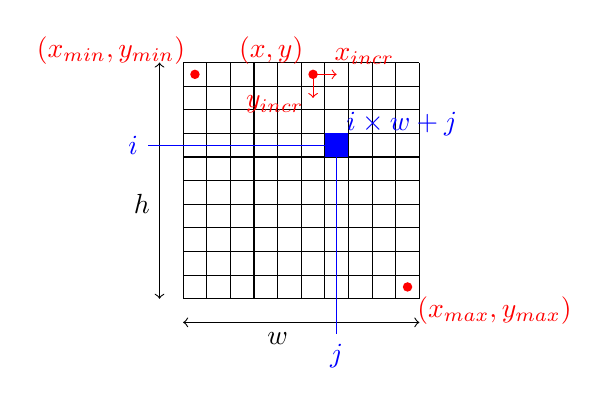
\begin{tikzpicture}[scale=0.3]
    % Colonnes
    \foreach \x in {-5, ..., 5} {
      \draw[thin] (\x, -5) -- (\x, 5);
    }
    % Lignes
    \foreach \y in {-5, ..., 5} {
      \draw[thin] (-5, \y) -- (5, \y);
    }

    % Dimensions
    \draw[<->] (-6, -5) -- (-6, 5) node[left, pos=0.4] {$h$};
    \draw[<->] (-5, -6) -- (5, -6) node[below, pos=0.4] {$w$};

    % Mon pixel
    \fill[blue] (2, 2) -- ++(-1, 0) -- ++(0, -1) -- ++ (1, 0) --
    cycle;
    \draw[blue] (1, 1.5) -- (-6.5, 1.5) node[left, blue] {$i$};
    \draw[blue] (1.5, 1) -- (1.5, -6.5) node[below, blue] {$j$};
    \node[blue, above right] at (1.5, 1.5) {$i \times w + j$};

    % Plan complexe
    \fill[red] (-4.5, 4.5) circle [radius=0.2] node[red, above left]
    {$(x_{min}, y_{min})$};
    \fill[red] (4.5, -4.5) circle [radius=0.2] node[red, below right]
    {$(x_{max}, y_{max})$};

    % Mon point complexe
    \coordinate (monpt) at (0.5, 4.5);
    \fill[red] (monpt) circle [radius=0.2] node[red, above left]
    {$(x, y)$};
    \draw[red, ->] (monpt) -- ++(1, 0) node[red, above right, pos=0.5]
    {$x_{incr}$};
    \draw[red, ->] (monpt) -- ++(0, -1) node[red, below left, pos=0.5]
    {$y_{incr}$};
  \end{tikzpicture}

  \caption{Paramètres de l'image dans le plan complexe}
  \label{fig:image-parameters}
\end{figure}

%\attention

% On fait un découpage par ligne parce que 
% plus facile
% moins de  communications

%%% Local Variables:
%%% mode: latex
%%% TeX-master: "../rapport"
%%% End:
